% Options for packages loaded elsewhere
\PassOptionsToPackage{unicode}{hyperref}
\PassOptionsToPackage{hyphens}{url}
\PassOptionsToPackage{dvipsnames,svgnames,x11names}{xcolor}
\documentclass[
]{article}
\usepackage{xcolor}
\usepackage[margin=1in]{geometry}
\usepackage{amsmath,amssymb}
\setcounter{secnumdepth}{-\maxdimen} % remove section numbering
\usepackage{iftex}
\ifPDFTeX
  \usepackage[T1]{fontenc}
  \usepackage[utf8]{inputenc}
  \usepackage{textcomp}
  \DeclareUnicodeCharacter{03B7}{$\eta$}
  \DeclareUnicodeCharacter{2264}{$\leq$}
  \DeclareUnicodeCharacter{2212}{$-$}
  \DeclareUnicodeCharacter{2078}{\textsuperscript{8}}
  \DeclareUnicodeCharacter{2079}{\textsuperscript{9}}
  \DeclareUnicodeCharacter{2192}{$\rightarrow$}
  \usepackage{textcomp} % provide euro and other symbols
\else % if luatex or xetex
  \usepackage{unicode-math} % this also loads fontspec
  \defaultfontfeatures{Scale=MatchLowercase}
  \defaultfontfeatures[\rmfamily]{Ligatures=TeX,Scale=1}
\fi
\usepackage{lmodern}
\ifPDFTeX\else
  % xetex/luatex font selection
\fi
% Use upquote if available, for straight quotes in verbatim environments
\IfFileExists{upquote.sty}{\usepackage{upquote}}{}
\IfFileExists{microtype.sty}{% use microtype if available
  \usepackage[]{microtype}
  \UseMicrotypeSet[protrusion]{basicmath} % disable protrusion for tt fonts
}{}
\makeatletter
\@ifundefined{KOMAClassName}{% if non-KOMA class
  \IfFileExists{parskip.sty}{%
    \usepackage{parskip}
  }{% else
    \setlength{\parindent}{0pt}
    \setlength{\parskip}{6pt plus 2pt minus 1pt}}
}{% if KOMA class
  \KOMAoptions{parskip=half}}
\makeatother
\usepackage{longtable,booktabs,array}
\usepackage{calc} % for calculating minipage widths
% Correct order of tables after \paragraph or \subparagraph
\usepackage{etoolbox}
\makeatletter
\patchcmd\longtable{\par}{\if@noskipsec\mbox{}\fi\par}{}{}
\makeatother
% Allow footnotes in longtable head/foot
\IfFileExists{footnotehyper.sty}{\usepackage{footnotehyper}}{\usepackage{footnote}}
\makesavenoteenv{longtable}
\usepackage{graphicx}
\makeatletter
\newsavebox\pandoc@box
\newcommand*\pandocbounded[1]{% scales image to fit in text height/width
  \sbox\pandoc@box{#1}%
  \Gscale@div\@tempa{\textheight}{\dimexpr\ht\pandoc@box+\dp\pandoc@box\relax}%
  \Gscale@div\@tempb{\linewidth}{\wd\pandoc@box}%
  \ifdim\@tempb\p@<\@tempa\p@\let\@tempa\@tempb\fi% select the smaller of both
  \ifdim\@tempa\p@<\p@\scalebox{\@tempa}{\usebox\pandoc@box}%
  \else\usebox{\pandoc@box}%
  \fi%
}
% Set default figure placement to htbp
\def\fps@figure{htbp}
\makeatother
\usepackage{svg}
\setlength{\emergencystretch}{3em} % prevent overfull lines
\providecommand{\tightlist}{%
  \setlength{\itemsep}{0pt}\setlength{\parskip}{0pt}}
\usepackage{bookmark}
\IfFileExists{xurl.sty}{\usepackage{xurl}}{} % add URL line breaks if available
\urlstyle{same}
\hypersetup{
  colorlinks=true,
  linkcolor={blue},
  filecolor={Maroon},
  citecolor={Blue},
  urlcolor={Blue},
  pdfcreator={LaTeX via pandoc}}

\author{}
\date{}

\begin{document}

\section{Direct Energy Conversion for Fusion: Fuel, Confinement, and the
Cost
Question}\label{direct-energy-conversion-for-fusion-fuel-confinement-and-the-cost-question}

Every fusion power plant has to turn plasma energy into electricity. The
default path is thermal: fusion power heats a working fluid that runs
through a turbine to spin a generator. Turbines and generators convert
heat to power in virtually every coal, gas, and fission plant on the
grid. A steam Rankine cycle runs at 35-40\%, a supercritical CO2 Brayton
cycle at 47\%, and a combined cycle at 53\%. These are mature technology
with known capital costs.

The thermal conversion default has two drawbacks. Physics sets a low
efficiency ceiling, and its hardware is expensive. Direct energy
conversion (DEC) is used loosely here for any architecture that skips
the heat cycle, the turbine, or both. Solar photovoltaics (PV) skip
both, turning photons directly into current. Wind and hydro skip just
the heat cycle, converting kinetic energy through a turbine to
electricity. MHD generators skip just the turbine, extracting current
from a conducting fluid in a magnetic field.

Fusion DEC skips both: turn charged plasma particles directly into
current by decelerating them against an electric potential, or by
inducing current in surrounding coils as the plasma expands. Whether
that works, and how much of the fusion power it captures, depends on the
fuel and the confinement. DEC only pays off when most of the fusion
energy comes out as charged particles, which rules out D-T (80\%
neutrons) and makes p-B11 marginal (87-97\% bremsstrahlung). D-He3 is
the natural fit (20-30\% bremsstrahlung, 5\% neutrons).

Different confinements need different capture hardware: venetian-blind
grids for mirrors, inductive coils for pulsed concepts. This post walks
through three DEC paths, what each would need to deliver, and where the
room to run actually is. The costing framework builds on our
\href{https://1cf.energy/fusions-cost-floor-what-if-the-core-were-free/}{prior
analysis} of the industrial floor on fusion electricity cost; we
reference it when free-core numbers appear, but this piece stands alone.

\subsection{What Direct Energy Conversion
Does}\label{what-direct-energy-conversion-does}

The Carnot limit bounds any heat engine, η ≤ 1 − T\_cold/T\_hot. In a
fusion plant the hot-side temperature is capped by what first-wall and
blanket materials can tolerate (500-700°C for RAFM steel and SiC
composites), which puts the Carnot ceiling around 60-65\% against a 300
K cold sink; real cycles give back another 10-15 points to
heat-exchanger and turbine irreversibilities, which is why sCO2 Brayton
sits at 47\% and combined cycle at 53\%. DEC is bounded too, but much
more loosely: the effective ``hot side'' for a fusion plasma sits at
10⁸-10⁹ K, so the Carnot-equivalent ceiling is essentially 100\%. The
remaining gap to that ceiling is engineering, not thermodynamics. The
gap of roughly 50 percentage points between thermal and DEC is why DEC
is interesting in principle. Whether it pays off in practice is the
question this post takes up.

Fusion DEC only works on charged particles. Neutrons carry no charge,
and photons at keV bremsstrahlung energies have no demonstrated fusion
DEC path; TAE's proposed X-ray capture scheme via cascading Auger
emission
(\href{https://patents.google.com/patent/US9893226B2/}{Binderbauer \&
Tajima, 2018}) remains untested (see ``The Bremsstrahlung Constraint''
below). DEC therefore requires fuel where most of the energy is in
charged particles: deuterium-helium-3 (5\% of fusion energy in neutrons)
or proton-boron (0.2\% neutrons). Deuterium-tritium (80\% neutrons) is
not a DEC fuel.

Photons aren't a nuclear constraint, but at fusion temperatures they can
be debilitating. For p-B11, the high plasma temperature (\textgreater100
keV) and Z=5 boron drive intense bremsstrahlung: roughly 97\% of fusion
power in a thermonuclear plasma, leaving a 3\% margin
(\href{https://doi.org/10.1088/1741-4326/ab1a60}{Putvinski et al.,
2019}). Driving the plasma out of equilibrium widens the margin to about
13\% (\href{https://doi.org/10.1103/PhysRevE.106.055215}{Ochs et al.,
2022}), but photons still carry 87\%. They hit the walls as heat. DEC
handles the charged-particle margin; the thermal plant handles the rest.

\begin{longtable}[]{@{}lllll@{}}
\toprule\noalign{}
Channel & D-T & D-³He & p-¹¹B (thermal) & p-¹¹B (non-thermal) \\
\midrule\noalign{}
\endhead
\bottomrule\noalign{}
\endlastfoot
Neutrons & 80\% & 5\% & 0.2\% & 0.2\% \\
Bremsstrahlung / X-ray & small & 25\% & 97\% & 87\% \\
Extractable charged & 20\% & 70\% & 3\% & 13\% \\
Total energy per reaction & 17.6 MeV & 18.3 MeV & 8.7 MeV & 8.7 MeV \\
\end{longtable}

\begin{figure}
\centering
\pandocbounded{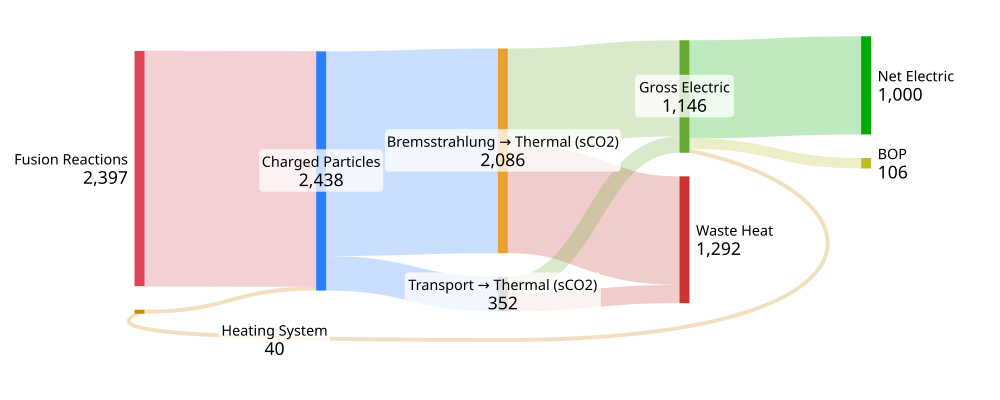
\includegraphics[keepaspectratio]{p-B11 Thermal Cycle.pdf}}
\caption{Power flow in a 1 GWe p-B11 thermal-only mirror: 87\% of fusion
power (2,086 MW) is re-radiated as bremsstrahlung, 13\% (352 MW) escapes
as charged-particle transport, and both feed a single sCO2 turbine at
47\%.}
\end{figure}

\subsection{Three Paths to Fusion DEC}\label{three-paths-to-fusion-dec}

\subsubsection{Venetian Blind}\label{venetian-blind}

The
\href{https://iopscience.iop.org/article/10.1088/0029-5515/13/1/005}{venetian
blind} is the most mature DEC concept (TRL 4-5). It consists of angled
metal ribbon grids at successively higher retarding potentials that sort
ions by energy and collect them on high-potential electrodes. It mounts
on linear magnetic confinement devices such as magnetic mirrors, as an
add-on to the expander tank, collecting the particle stream leaving
along field lines. It has no moving parts, and was
\href{https://doi.org/10.13182/FST83-A20820}{demonstrated at 48\%
efficiency} on real end-loss plasma at LLNL's TMX (Barr \& Moir, 1983), with a
\href{https://iopscience.iop.org/article/10.1088/0029-5515/13/1/005}{theoretical
maximum of 70\%}. The 70\% cap is set by grid geometry and the ion
energy spread, not by the wall-material Carnot limit.
\href{https://www.realtafusion.com/}{Realta Fusion} is the sole active
developer, with a
\href{https://patents.google.com/patent/US12166398B2}{patented}
axisymmetric variant.

\subsubsection{Pulsed Inductive}\label{pulsed-inductive}

Pulsed inductive DEC is a less-mature DEC concept (TRL 3 for fusion
use). It consists of coils surrounding a compression chamber that
compress a pulsed plasma and then recover energy as it re-expands,
inducing current via Faraday's law, requiring no plasma-surface contact;
the same coils drive both halves of the cycle. No published
demonstration on fusion plasma yet. Helion
\href{https://www.helionenergy.com/}{claims 95\%} electrical round-trip
efficiency on the capacitor → compression → plasma → expansion →
recovery-capacitor cycle, measured at pre-fusion conditions (plasma
compressed, no net fusion gain). The
\href{https://youtu.be/5nHmqk1cI2E?t=505}{theoretical framework}
(Kirtley et al., APS DPP 2024) suggests 68-87\% for reactor-relevant
pulses. This range is set by pulse-cycle losses, not by the
wall-material Carnot limit. \href{https://www.helionenergy.com/}{Helion
Energy} is the sole
\href{https://doi.org/10.1088/0029-5515/51/5/053008}{active developer},
using D-He3 FRC plasmoids that collide and merge in the compression
chamber; Polaris (Helion's seventh device, under construction) is
designed to measure round-trip efficiency on plasma.

\subsubsection{MHD Generator}\label{mhd-generator}

A \href{https://inis.iaea.org/records/4ss3z-rqd83}{magnetohydrodynamic
generator} passes a conducting fluid through a transverse magnetic
field, driving current through electrodes via the Lorentz force. No
moving parts. From the 1960s through 1993, the US, Soviet, Japanese, and
Australian governments
\href{https://www.gao.gov/products/emd-80-14}{spent hundreds of
millions} developing MHD generators on hot coal combustion gas,
demonstrating up to \href{https://www.osti.gov/biblio/6380343}{32 MW
gross output} at TRL 5-6. Liquid-metal MHD (LMMHD) has separately shown
\href{https://doi.org/10.1016/0196-8904(81)90006-6}{\textgreater71\%
efficiency} at small scale; projected efficiency for LMMHD on fusion
coolants is \textgreater60\%.

MHD is not a charged-particle DEC; it replaces the Brayton turbine, not
the heat cycle, and is still Carnot-limited. Any fusion plant could
route its coolant through an MHD channel instead of a turbine. For D-T,
LMMHD integrated into the lithium breeding blanket handles neutron and
thermal energy. For aneutronic fuels, it handles the bremsstrahlung
fraction that charged-particle DEC cannot touch. The obstacle is that no
fusion-MHD system has ever been built. The problem that killed the coal
programs (\href{https://www.gao.gov/products/emd-80-14}{electrode
erosion from coal slag}) doesn't apply to clean fusion coolants, but a
new one appears: MHD pressure drop, where liquid metal flowing through
fusion-scale magnetic fields (5-15 T) experiences enormous drag,
potentially consuming more pumping power than the MHD generates. This is
an \href{https://doi.org/10.3390/en14206640}{active research problem} at
ORNL and KIT Karlsruhe, with no demonstrated solution at reactor scale.
For this analysis, MHD remains a what-if: promising physics, no costable
design.

\subsection{Modeled Approaches}\label{modeled-approaches}

We modeled two DEC architectures (venetian blind hybrid and pulsed
inductive) with a free fusion core, using the same methodology as the
\href{https://1cf.energy/fusions-cost-floor-what-if-the-core-were-free/}{previous
dispatch}. Numbers can be reproduced with the
\href{https://github.com/1cfe/1costingfe/blob/master/examples/dec_blog_numbers.py}{companion
script}.

One caveat up front: the thermal capture hardware in the baseline
(turbine island, generator, sCO2 Brayton loop) draws on a century of
manufacturing cost-down, thousands of GW deployed, and well-understood
NOAK pricing. The DEC estimates rest on much thinner ground: 1977
EPRI/LLNL studies for the venetian blind, and a single developer's
capacitor build-up for the pulsed inductive. Both sit closer to FOAK
than the turbine they displace. The cost tables below compare them
head-to-head today; the Learning Rates section returns to what DEC could
look like once that gap closes.

\subsubsection{Venetian Blind + Thermal Hybrid
~(p-B11)}\label{venetian-blind-thermal-hybrid-p-b11}

We carry the p-B11 mirror baseline forward from the
\href{https://1cf.energy/fusions-cost-floor-what-if-the-core-were-free/}{prior
dispatch} and add a venetian blind as an overlay. The thermal cycle is
kept because 87\% of p-B11 energy radiates as bremsstrahlung; the DEC
captures only the charged-particles leaving the mirror axially.

Sizing the VB hardware to 400 MWe DEC output (2024 NOAK) lands an
all-in figure of roughly \$140M, range \$105--190M: a 304L stainless
tank (\$8--12/kg fabricated, 1500--3000 tonnes, \textasciitilde\$20M),
HV power conditioning at \$100--120/kW (60--70\% of a full
\href{https://cdn.misoenergy.org/20240501\%20PSC\%20Item\%2004\%20MISO\%20Transmission\%20Cost\%20Estimation\%20Guide\%20for\%20MTEP24632680.pdf}{MISO
2024 VSC HVDC station} since the AC interconnect isn't duplicated,
\textasciitilde\$45M), cryopumps at fusion procurement scale
(\textasciitilde\$15M), ITER NBI-style actively cooled thermal panels
for the 30--90 MW grid heat load (\textasciitilde\$15M), grid and
collector hardware (\textasciitilde\$15M, Hoffman 1977 geometry x CPI),
HV bushings, valves, and controls (\textasciitilde\$12M), plus 15\%
installation. This is comparable to the turbine island it partially
replaces (\$168M for sCO2 at 1 GWe).

We model the hybrid with DEC handling 90\% of the charged particle
transport and the rest going through a small thermal cycle:

\begin{longtable}[]{@{}
  >{\raggedright\arraybackslash}p{(\linewidth - 4\tabcolsep) * \real{0.3333}}
  >{\raggedright\arraybackslash}p{(\linewidth - 4\tabcolsep) * \real{0.3333}}
  >{\raggedright\arraybackslash}p{(\linewidth - 4\tabcolsep) * \real{0.3333}}@{}}
\toprule\noalign{}
\begin{minipage}[b]{\linewidth}\raggedright
Configuration (1 GWe, pB11, free core)
\end{minipage} & \begin{minipage}[b]{\linewidth}\raggedright
Floor (\$/MWh)
\end{minipage} & \begin{minipage}[b]{\linewidth}\raggedright
Overnight (\$/kW)
\end{minipage} \\
\midrule\noalign{}
\endhead
\bottomrule\noalign{}
\endlastfoot
Thermal only (sCO2 Brayton, 47\%) & 18 & 1,250 \\
VB DEC at 48\% + thermal (hybrid) & 19 & 1,264 \\
VB DEC at 60\% + thermal (hybrid) & 19 & 1,261 \\
\end{longtable}

The venetian blind barely moves the floor. With 87\% of fusion energy
radiated as bremsstrahlung, the DEC only captures the 13\%
charged-particle margin. At the demonstrated 48\% efficiency, the DEC
hardware adds cost without meaningfully improving conversion. Even at
60\% (never demonstrated on real plasma), the hybrid floor sits at
\$19/MWh, \$1/MWh above thermal-only and about \$11--14/kW worse on
overnight. Eliminating the turbine entirely and wasting the
bremsstrahlung is not viable for p-B11: without a thermal cycle, the
plant needs 16 GW of fusion power for 1 GWe net, driving the fully
costed LCOE to \$60/MWh, far worse than the thermal path (\$37/MWh). For
D-He3 with its higher charged fraction, the VB DEC 60\% floor is
\$16/MWh, but the He-3 fuel adds \$72/MWh on top.

The numbers above use the mirror baseline heating power of 40 MW,
giving Q\_eng around 8 and a 13\% recirculating fraction. If the
heating power is larger, the picture shifts. The heating power leaves
the plasma in the charged-particle transport channel, and is mostly
captured by the VB. But at a heating wall-plug efficiency of 50\% (the
model's NBI default) the injection chain draws 2 MW of gross electric
per 1 MW delivered to the plasma, while the transport channel returns
only 0.58 MW in the VB 60\% hybrid. Each MW of heating therefore costs
roughly 1.4 MW of gross electric output (2 MW drawn in, 0.58 MW
returned), and the fusion core upsizes to cover the shortfall. Holding
net output at 1 GWe, LCOE rises by \$1/MWh at 150 MW heating, by
\$3/MWh at 250 MW, and by \$5/MWh at 400 MW; beyond 600 MW Q\_eng
drops below 2 and the recirculating fraction exceeds 50\%. Thermal-only
stays cheaper than the thermal+VB hybrid by about \$0.9/MWh at every
heating level: the VB hardware cost scales with DEC throughput
alongside the recovery it provides, so the gap stays roughly flat
across the sweep.

Flipping the analysis: at fixed VB hardware cost, what efficiency
would justify adding the DEC? At the 1 GWe p-B11 baseline the VB only
outputs roughly 145 MWe (13\% charged fraction of 2 GW fusion, 90\%
captured, 60\% converted), so the build-up scales to about \$81M of VB
hardware at this plant scale. Holding that fixed, no VB efficiency
between 30\% and 100\% breaks even with thermal-only --- the VB
hardware exceeds turbine-side savings across the entire physically
accessible band, and even at a hypothetical 100\% VB efficiency the
hybrid is still about \$0.3/MWh above thermal-only. Break-even enters
the physically accessible window only if the VB capex at this plant
scale falls by roughly 3x, to around \$30M, at which point a 62\% VB
suffices. The leverage is narrow: only 12\% of fusion power (0.9 x
0.13) flows through the DEC, so each percentage point of VB efficiency
moves only 0.12 percentage points of plant-level conversion.

\subsubsection{Pulsed Inductive (D-He3)}\label{pulsed-inductive-d-he3}

Pulsed inductive DEC using D-He3 plasma is Helion's concept. Helion is
one of the best-capitalized American fusion companies (roughly \$1.8B
raised) and has signed a
\href{https://www.microsoft.com/en-us/blog/2023/05/10/microsoft-signs-agreement-with-helion-energy-to-purchase-electricity/}{commercial
PPA with Microsoft} targeting 2028. D-He3 radiates only 25\% of its
energy as bremsstrahlung, leaving most of the fusion power to the
charged particles and the inductive coils. Unlike the VB hybrid, no main
turbine is retained; the pulsed-power chain handles most of the
conversion, with a small thermal bottoming cycle for the bremsstrahlung
and neutron fractions.

With no turbine, the BOP becomes a pulsed-power chain: pulse-rated
switchgear, capacitor or inductive storage to smooth the duty cycle,
DC-DC converters to recharge the compression coils, and a grid-tie
inverter at the back. A utility-scale solar inverter (\$30-50/kWdc,
\href{https://docs.nrel.gov/docs/fy25osti/92536.pdf}{NREL Table A-3})
is only the last link. Sizing the pulsed chain downstream of the driver
to 1 GWe net (NOAK) gives a defensible all-in figure of roughly
\$593/kW: a dedicated recovery cap bank sized to the fusion power
balance (703 MJ at \$0.50/J = \$351M), DC-DC links at \$75/kW of gross
output (\$78M), the grid inverter at \$150/kW net (\$150M), and controls
at 4\% of the driver bank (\$14M). The compression bank itself (\$351M)
is accounted for as part of the driver (core).

\begin{longtable}[]{@{}
  >{\raggedright\arraybackslash}p{(\linewidth - 6\tabcolsep) * \real{0.2500}}
  >{\raggedright\arraybackslash}p{(\linewidth - 6\tabcolsep) * \real{0.2500}}
  >{\raggedright\arraybackslash}p{(\linewidth - 6\tabcolsep) * \real{0.2500}}
  >{\raggedright\arraybackslash}p{(\linewidth - 6\tabcolsep) * \real{0.2500}}@{}}
\toprule\noalign{}
\begin{minipage}[b]{\linewidth}\raggedright
Configuration (1 GWe, D-He3, free core)
\end{minipage} & \begin{minipage}[b]{\linewidth}\raggedright
BOP floor (\$/MWh)
\end{minipage} & \begin{minipage}[b]{\linewidth}\raggedright
He-3 fuel (\$/MWh)
\end{minipage} & \begin{minipage}[b]{\linewidth}\raggedright
Total (\$/MWh)
\end{minipage} \\
\midrule\noalign{}
\endhead
\bottomrule\noalign{}
\endlastfoot
Thermal only (sCO2 Brayton, 47\%) & 19 & 80 & 99 \\
Pulsed inductive (85\% η, no turbine) & 24 & 55 & 78 \\
\end{longtable}

The BOP floor comes in \$5/MWh above thermal: \$24/MWh vs \$19/MWh. The
turbine island is not the dominant cost. Buildings (\$354M), the
electrical plant (\$96M), O\&M (\$37M/yr), and financing charges
together dwarf the turbine, and the pulsed-power chain that replaces it
costs more than the turbine. Eliminating the turbine and its synchronous
generator (including the GSU transformer and sync/protection gear)
removes about \$186M of overnight capital, but the \$593M of
pulsed-power hardware needed to shape, store, and grid-tie the recovered
energy more than offsets those savings.

The He-3 fuel cost is a different problem. At \$2M/kg (optimistic), He-3
adds \$55/MWh, more than five times the 1-cent target by itself. At the
\href{https://www.everycrsreport.com/reports/R41419.html}{DOE-allocated
price} of \$4.5M/kg, it roughly doubles. Helion's answer is to breed
He-3 internally from D-D side reactions. If the fuel cost drops to zero,
the D-He3 pulsed DEC floor sits at \$24/MWh, still above thermal
(\$19/MWh) and well above the 1-cent target.

The round-trip efficiency of the compression-expansion cycle is the
other open question. Helion \href{https://www.helionenergy.com/}{claims
95\%} but has not published data. The
\href{https://youtu.be/5nHmqk1cI2E?t=505}{theoretical framework}
(Kirtley et al., APS DPP 2024) suggests 68--87\% is more realistic for
plasma-present operation, depending on the burn cycle. At the modeled
85\%, the halving of fusion power and He-3 burn is what carries the
architecture, not the BOP hardware, which already costs more than a
turbine. At 70\%, the core-size and fuel savings shrink and the pulsed
chain looks clearly worse than a turbine. Below 60\%, the economics
plainly favor just building a turbine.

\begin{figure}
\centering
\pandocbounded{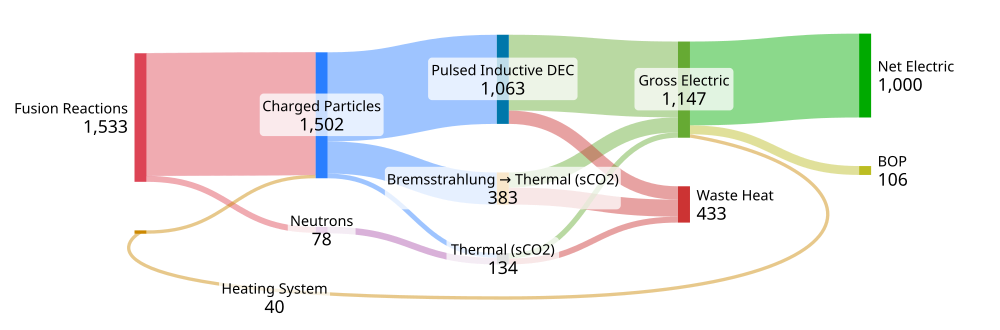
\includegraphics[keepaspectratio]{D-He3 Pulsed Inductive DEC.pdf}}
\caption{Power flow in a 1 GWe D-He3 mirror with pulsed inductive DEC at
85\%: 95\% of charged-particle transport (1,063 MW of 1,119 MW) drives
the DEC, while bremsstrahlung (25\% of fusion power) and neutrons drive
a thermal bottoming cycle.}
\end{figure}

\subsection{What the Floor Is, and
Isn't}\label{what-the-floor-is-and-isnt}

Here is the comparison at aggressive conditions (2 GWe, 95\%
availability, 3\% WACC, 50-year life, 3-year construction) where every
parameter is pushed:

\begin{longtable}[]{@{}
  >{\raggedright\arraybackslash}p{(\linewidth - 6\tabcolsep) * \real{0.2500}}
  >{\raggedright\arraybackslash}p{(\linewidth - 6\tabcolsep) * \real{0.2500}}
  >{\raggedright\arraybackslash}p{(\linewidth - 6\tabcolsep) * \real{0.2500}}
  >{\raggedright\arraybackslash}p{(\linewidth - 6\tabcolsep) * \real{0.2500}}@{}}
\toprule\noalign{}
\begin{minipage}[b]{\linewidth}\raggedright
Approach (2 GWe, pB11, free core)
\end{minipage} & \begin{minipage}[b]{\linewidth}\raggedright
Floor (\$/MWh)
\end{minipage} & \begin{minipage}[b]{\linewidth}\raggedright
Overnight (\$/kW)
\end{minipage} & \begin{minipage}[b]{\linewidth}\raggedright
Budget for core
\end{minipage} \\
\midrule\noalign{}
\endhead
\bottomrule\noalign{}
\endlastfoot
Thermal only (sCO2 Brayton, 47\%) & 7.6 & 826 & +\$2.4/MWh \\
VB DEC 60\% + thermal (hybrid) & 7.9 & 861 & +\$2.1/MWh \\
\end{longtable}

At aggressive conditions, the hybrid DEC and thermal approaches are
within \$0.2/MWh. The no-turbine configurations are excluded for p-B11
because wasting 87\% of fusion energy as bremsstrahlung heat requires an
enormous core that more than offsets the turbine savings (see above).
The dominant terms remain buildings (\$370-490M), the electrical plant
(\$180M), O\&M (\$62M/yr), indirect costs, and financing.

The floor is not set by the power conversion choice. It is set by the
industrial cost of building, staffing, and financing a large power
plant. DEC's value, if any, has to show up somewhere else: on the core,
on the fuel, or on the efficiency ceiling.

\subsection{Where DEC Pays Off}\label{where-dec-pays-off}

If DEC doesn't move the floor, why does it matter?

The floor is what you pay with a free fusion core. The core is not free.
DEC's real benefit is that higher conversion efficiency means
\textbf{you need less fusion power for the same net electric output},
and for D-He3, less fusion power also means less He-3 fuel consumed.

In the fully costed D-He3 mirror at 1 GWe baseline conditions:

\begin{longtable}[]{@{}llll@{}}
\toprule\noalign{}
Configuration & LCOE (\$/MWh) & Core cost & He-3 fuel (\$/MWh) \\
\midrule\noalign{}
\endhead
\bottomrule\noalign{}
\endlastfoot
Thermal only (47\%) & 120 & \$1,315M & 80 \\
VB DEC 60\% (hybrid) & 110 & \$1,353M & 72 \\
Pulsed inductive (85\%) & 95 & \$1,696M & 55 \\
\end{longtable}

For the venetian blind, the core cost rises modestly (\$38M): the added
DEC hardware partially offsets the savings from smaller heating and
blanket systems. For pulsed inductive, the core jumps \$381M because
the pulsed-power chain that replaces the turbine (dominated by the
recovery cap bank) is substantial. LCOE drops \$10/MWh with the
venetian blind and \$25/MWh with pulsed inductive, but the pulsed
savings come entirely from fuel, not hardware: higher efficiency means
less fusion power per MWh, which means less He-3 burned. For D-He3,
DEC is primarily a fuel-saving technology.

For p-B11 (negligible fuel cost), the effect is smaller: thermal LCOE is
\$37/MWh, VB DEC 60\% is \$37/MWh (core \$1,202M vs \$1,235M). Because
bremsstrahlung dominates, the DEC captures only the 13\%
charged-particle margin and does not meaningfully reduce the required
fusion power.

The pulsed inductive case already costs more than a turbine on BOP even
at 85\% efficiency; the LCOE win over thermal comes entirely from
halving the fusion power and the He-3 burn. If the efficiency is 70\%
instead of 85\%, the core-size savings shrink and the pulsed power
system (capacitor banks, switches; the model assumes \$0.50/J stored
NOAK, vs \href{https://arxiv.org/abs/2602.19389}{\$2-4/J} in the
literature) becomes clearly more expensive than the turbine it replaces.
Capacitor lifetime is a separate risk: the model assumes 10\^{}8 shot
lifetime (NOAK), but current high-energy-density capacitors achieve
roughly 10\^{}7 cycles. At a 1 Hz rep rate, 10\^{}7 shots is four months
of operation, requiring frequent bank replacements that add both capital
cost and downtime.

\subsection{The Bremsstrahlung
Constraint}\label{the-bremsstrahlung-constraint}

Every charged-particle DEC architecture for p-B11 runs into
bremsstrahlung. As noted above, even in the most favorable scenario,
bremsstrahlung is 87\% of fusion power. Without driving the plasma out
of equilibrium, the margin is only 3\%.

This is more severe than the previous dispatch acknowledged. In a p-B11
plant, charged-particle DEC captures the margin; radiation handles the
majority. The thermal plant is not a small bottoming cycle; it is the
primary power conversion pathway.

The options for the radiated fraction are:

\begin{enumerate}
\def\labelenumi{\arabic{enumi}.}
\tightlist
\item
  \textbf{Thermal cycle}: a full turbine island converts bremsstrahlung
  heat at 47--53\%. This is what the ``hybrid'' configurations above
  assume. It works but preserves essentially the full thermal BOP.
\item
  \textbf{MHD on the coolant}: if the bremsstrahlung-heated wall coolant
  is liquid metal, an MHD channel could convert at \textgreater60\% with
  no turbine. Undemonstrated at reactor scale.
\item
  \textbf{Reject as waste}: accept the efficiency loss and dump the
  bremsstrahlung heat to cooling towers. At 87\% bremsstrahlung
  fraction, this means wasting most of the fusion energy. The overall
  plant efficiency collapses: a DEC at 85\% efficiency on the 13\% net
  charged fraction yields only 11\% of fusion power as electricity, far
  worse than thermal-only (47\%).
\item
  \textbf{X-ray photovoltaic DEC}: convert bremsstrahlung directly to
  electricity via cascading Auger emission in nanometric high-Z/low-Z
  layers
  (\href{https://patents.google.com/patent/US9893226B2/}{Binderbauer \&
  Tajima, 2018}). If it works, this would capture the bremsstrahlung
  fraction without a thermal cycle, but no prototype has been built, no
  efficiency has been measured, and the radiation damage environment
  (keV photons at GW/m² flux for years) is extreme. This is a TRL 1
  concept.
\end{enumerate}

Options 3 and 4 do not have a demonstrated path. Today, the thermal
plant is the only demonstrated path for the radiated fraction. DEC,
where it applies, captures only the charged-particle margin.

\begin{figure}
\centering
\pandocbounded{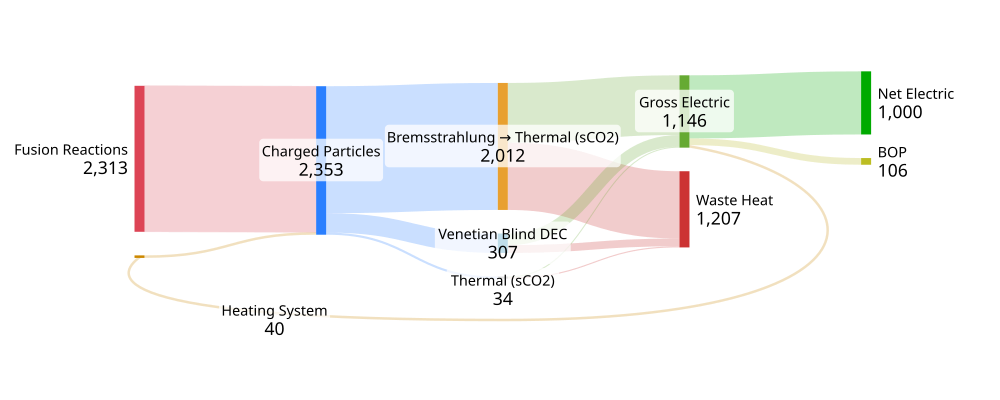
\includegraphics[keepaspectratio]{p-B11 VB DEC.pdf}}
\caption{Power flow in a 1 GWe p-B11 mirror with a venetian-blind DEC at
60\% hybrid with a thermal cycle: 87\% of fusion power (2,012 MW)
radiates as bremsstrahlung and feeds the turbine, while the DEC captures
only the 13\% charged-particle margin (307 MW).}
\end{figure}

\subsection{Learning Rates}\label{learning-rates}

The numbers above are snapshots. Deployed technologies get cheaper.
Turbines have been manufactured for over a century with thousands of GW
deployed; there is little room for costs to fall. The DEC concepts are
much lower TRL, with larger cost uncertainties but more room for
learning.

The venetian blind is the most mature DEC. Its dominant costs (vacuum
vessels, cryopumps) are mature industrial hardware, 75\% of total cost.
The grids are 2\%. Little room to learn down.

The pulsed inductive path is different. Capacitor banks and power
electronics dominate, and both are early in their deployment curves. The
\href{https://arxiv.org/abs/2602.19389}{NOAK assumption} in the
1costingfe model is \$0.50/J stored (all-in: capacitors, switches,
charging, buswork). Today's lab pricing is \$20--50/J, a 40--100x gap,
comparable to what solar PV achieved over two decades. Grid-tie
inverters have already followed that curve (\$1,000/kW in the early
2000s to \$100--150/kW today). But the fusion-specific components
(capacitors rated for 100 million cycles at high energy density) do not
yet exist as commercial products. The \$0.50/J figure is a target, not a
price anyone can buy today.

The pulsed floors in this post already assume the 40--100x reduction has
happened. If capacitors stay at \$5--20/J, those floors rise
substantially and the economics favor a turbine. The thermal and
venetian blind floors carry no comparable risk.

\pandocbounded{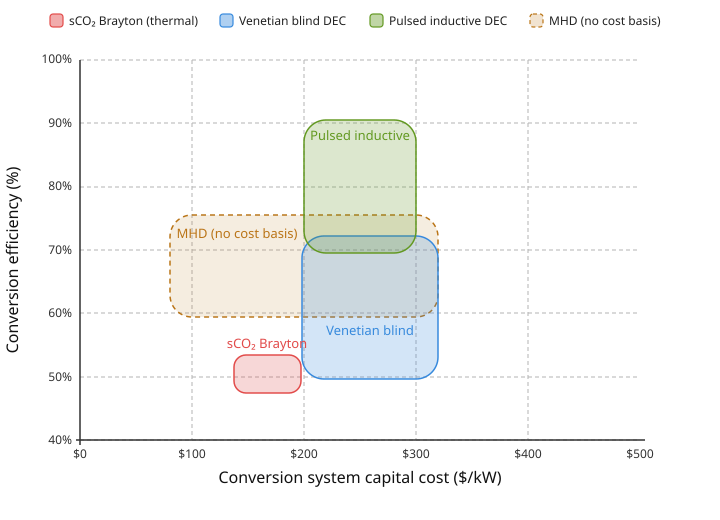
\includegraphics[keepaspectratio]{efficiency-cost chart.pdf}}

\subsection{Conclusions}\label{conclusions}

\textbf{1. DEC's potential value is efficiency, not BOP savings.} No DEC
has demonstrated efficiency above 48\% on real plasma, comparable to
sCO2 Brayton. If higher efficiencies are achieved, the payoff is a
smaller fusion core for the same net output. This shows up in the fully
costed plant, not the free-core floor.

\textbf{2. Power electronics ride a learning curve; turbines don't.}
Turbines have had a century of optimization and sit near their
asymptote. Capacitors, pulse-rated switchgear, and grid-tie conversion
sit on the same semiconductor and manufacturing-volume curves that took
solar PV and inverters from lab to commodity. Capacitor pricing has
roughly 40-100x to fall to hit the NOAK target used here, a reduction
comparable in magnitude to what PV achieved over two decades. DEC's cost
model has two levers that move in the right direction, efficiency and
unit cost; the thermal path has neither.

\textbf{3. The venetian blind has headroom.} At the demonstrated 48\%
efficiency, the DEC hardware costs about as much as the turbine it
replaces, with comparable conversion. The theoretical ceiling is 70\%,
with commercial efforts to close the gap underway at companies like
Realta. A sustained \textgreater60\% efficiency on real plasma is the
concrete milestone that would flip the venetian blind from even trade to
clear win.

\textbf{4. Pulsed inductive hinges on unverified efficiency; Polaris
will measure it.} If the round-trip efficiency is 85\%+, the pulsed
architecture halves the required fusion power and cuts He-3 burn
proportionally. The pulsed-power chain that replaces the turbine costs
more than a turbine, so BOP is more expensive than thermal; the savings
come from fuel and core size, not conversion hardware. If efficiency is
below 70\%, the fuel savings shrink and the higher BOP cost favors
building a turbine. The gap between viable and not sits in roughly 15
percentage points of unverified efficiency, which Polaris is expected to
measure on plasma.

\textbf{5. MHD generators could close the gap, someday.} An MHD
generator on the bremsstrahlung-heated coolant could convert the
radiated fraction at \textgreater60\% with no moving parts. The physics
is demonstrated; the engineering for fusion environments is not, with
liquid-metal MHD pressure drop at fusion field strengths the outstanding
problem.

\textbf{6. The p-B11 floor is industrial, not conversion-limited.} At
baseline conditions, the p-B11 cost floor is \$18/MWh regardless of
whether a venetian blind DEC is added. With 87\% of fusion energy
radiated as bremsstrahlung, the thermal plant handles the majority of
conversion and cannot be eliminated without an enormous increase in
fusion power. At aggressive conditions, thermal and hybrid DEC converge
to \$7.6-7.8/MWh. The floor is dominated by buildings, electrical
systems, O\&M, and financing, so DEC's leverage, if any, has to come
from elsewhere.

\textbf{7. For p-B11, alpha channeling or non-equilibrium operation is
the unlock.} DEC needs most fusion energy in charged particles, but
p-B11 radiates 87-97\% as bremsstrahlung. Thermonuclear operation leaves
a 3\% margin; driving the plasma out of equilibrium widens it to 13\%
(\href{https://doi.org/10.1103/PhysRevE.106.055215}{Ochs et al., 2022}).
The experimental program to demonstrate alpha channeling is what would
turn p-B11 DEC from a margin add-on into a real conversion path.

\textbf{8. D-He3 is the better DEC fuel, if you can get the He-3.} D-He3
has manageable bremsstrahlung (20-30\% of fusion power) and a large
charged fraction, making DEC a significant power path rather than a
margin add-on. But purchased He-3 costs \$55-80/MWh, far more than the
entire BOP floor. Self-breeding eliminates this, but whether a D-He3
device can breed enough He-3 to sustain itself is undemonstrated.

The path to 1-cent fusion energy does not run through direct energy
conversion alone. DEC does not remove the industrial cost structure that
creates the floor, and reaching \$10/MWh still requires the conditions
identified in the previous dispatch: large plants, high availability,
low-cost financing, fast construction, and long plant life. But DEC has
room to run in ways the thermal path does not. Three tractable
development targets would turn that room into numbers: venetian blind
efficiency sustained \textgreater60\% on real plasma, Helion's
round-trip demonstrated at 85\%+ on Polaris, and MHD pressure drop
solved at fusion field strengths. Each is an experimental program, not a
research miracle.

\subsection{References}\label{references}

\begin{enumerate}
\def\labelenumi{\arabic{enumi}.}
\tightlist
\item
  Moir, R.W. \& Barr, W.L., ``Venetian-blind direct energy converter for
  fusion reactors,'' \emph{Nuclear Fusion} 13, 35--45 (1973).
  \href{https://iopscience.iop.org/article/10.1088/0029-5515/13/1/005}{Link}
\item
  Hoffman, M.A., ``Electrostatic Direct Energy Converter Performance and
  Cost Scaling Laws,'' UCID-17560, LLNL (1977).
  \href{https://www.osti.gov/biblio/7218298}{Link}
\item
  Slough, J. et al., ``Creation of a high-temperature plasma through
  merging and compression of supersonic field reversed configuration
  plasmoids,'' \emph{Nuclear Fusion} 51(5), 053008 (2011).
  \href{https://doi.org/10.1088/0029-5515/51/5/053008}{Link}
\item
  Putvinski, S.V., Ryutov, D.D. \& Yushmanov, P.N., ``Fusion reactivity
  of the p-B11 plasma revisited,'' \emph{Nuclear Fusion} 59(7), 076018
  (2019). \href{https://doi.org/10.1088/1741-4326/ab1a60}{Link}
\item
  Ochs, I.E. et al., ``Improving the feasibility of economical
  proton-boron-11 fusion via alpha channeling with a hybrid fast and
  thermal proton scheme,'' \emph{Physical Review E} 106, 055215 (2022).
  \href{https://doi.org/10.1103/PhysRevE.106.055215}{Link}
\item
  Kirtley, D. et al., ``Generalized burn cycle efficiency framework,''
  APS DPP 2024, Abstract GO05.8.
  \href{https://youtu.be/5nHmqk1cI2E?t=505}{Presentation}
\item
  CATF IWG, ``Extension of the Fusion Power Plant Costing Standard,''
  arXiv:2602.19389 (2026). \href{https://arxiv.org/abs/2602.19389}{Link}
\item
  Rosa, R.J., \emph{Magnetohydrodynamic Energy Conversion}, Hemisphere
  Publishing (1987).
  \href{https://inis.iaea.org/records/4ss3z-rqd83}{Link}
\item
  GAO, ``Magnetohydrodynamics: A Promising Technology for Efficiently
  Generating Electricity From Coal,'' EMD-80-14 (1980).
  \href{https://www.gao.gov/products/emd-80-14}{Link}
\item
  Shea, D.A. \& Morgan, D., ``The Helium-3 Shortage: Supply, Demand, and
  Options for Congress,'' Congressional Research Service, R41419 (2010).
  \href{https://www.everycrsreport.com/reports/R41419.html}{Link}
\item
  Barr, W.L. \& Moir, R.W., ``Test Results on Plasma Direct Converters,''
  \emph{Fusion Technology} 3(1), 98-111 (1983).
  \href{https://doi.org/10.13182/FST83-A20820}{Link}
\item
  Fabris, G. \& Hantman, R.G., ``Interaction of fluid dynamics phenomena
  and generator efficiency in two-phase liquid-metal gas
  magnetohydrodynamic power generators,'' \emph{Energy Conversion and
  Management} 21(1), 49-60 (1981).
  \href{https://doi.org/10.1016/0196-8904(81)90006-6}{Link}
\item
  Pinkhasov, D. et al., ``CDIF 32-MWt MHD Program Results,'' \emph{Proc.
  31st Symposium on Engineering Aspects of MHD} (1993).
  \href{https://www.osti.gov/biblio/6380343}{Link}
\item
  Smolentsev, S. et al., ``MHD Thermofluid Issues of Liquid-Metal
  Blankets: Phenomena and Advances,'' \emph{Energies} 14(20), 6640
  (2021). \href{https://doi.org/10.3390/en14206640}{Link}
\item
  Binderbauer, M.W. \& Tajima, T., US Patent 9,893,226 B2,
  ``Photon-to-electric direct conversion'' (2018).
  \href{https://patents.google.com/patent/US9893226B2/}{Link}
\item
  Ramasamy, V. et al., ``Documenting 15 Years of Reductions in U.S.
  Solar Photovoltaic System Costs,'' NREL/TP-7A40-92536 (2025).
  \href{https://docs.nrel.gov/docs/fy25osti/92536.pdf}{Link}
\item
  Realta Fusion, US Patent 12,166,398 B2, ``Axisymmetric ferromagnetic
  venetian blinds'' (2025).
  \href{https://patents.google.com/patent/US12166398B2}{Link}
\item
  1cFE, ``1costingfe: Open-source fusion techno-economic model.''
  \href{https://github.com/1cfe/1costingfe}{GitHub}
\end{enumerate}

\end{document}
